%----------------------------------------
% Write your notes here
%----------------------------------------

usepackage{amsmath}

\section{Introduction}
Jake began the lecture by pointing out that our Homework 1 submissions were generally non-reproducible, and provided an overview of general practices to ensure reproducibility in Homework 2. We began our discussion in class with two main questions: \textbf{How should one evaluate research results?} and \textbf{Will the result hold up with new data but the same analysis?}.

\section{Crisis}
We looked at the paper \textbf{Estimating the reproducibility of psychological science} which was a broad research project undertaken by a large number of scientists. 100 experimental and correlational studies were replicated. Of the replicated studies, 36\% had statistically significant results whereas 97\% of the original studies had significant results in their original publications. Importantly, 47\% of the original effect sizes were in the 95\% confidence interval of the replication effect size, which leads us to conclude that we should believe about half of what we read in the psychological literature. 

\section{What is an Effect Size?}
So, what exactly is an effect size? 

In statistics, an effect size is a quantitative measure of the magnitude of a phenomenon. Examples of effect sizes are the correlation between two variables, the regression coefficient in a regression, the mean difference, or even the risk with which something happens, such as how many people survive after a heart attack for every one person that does not survive. Source: Wikipedia: Effect Size 

We looked at \url{https://rpsychologist.com/d3/cohend/} to visualize Effect Sizes. The visualization is designed to show the real meaning of a type of effect size popularly cited in psychology. The main takeaways of this animation is summarized in the following statement, "Factors like the quality of the study, the uncertainty of the estimate and results from previous work in the field need to be appraised before declaring an effect "large"." Importantly, when comparing a control and test group with each other, we should consider not only the mean difference, but also the difference in variance between the distributions being studied. 

\section{Misunderstandings in Statistics}

We looked at the paper, \textbf{Statistical tests, P values, confidence intervals, and power: a guide to misinterpretations} and worked on the following problem to clarify our understanding of the probability of real effects utilizing Bayes Rule. 

\begin{figure}[ht]
  \begin{center}
    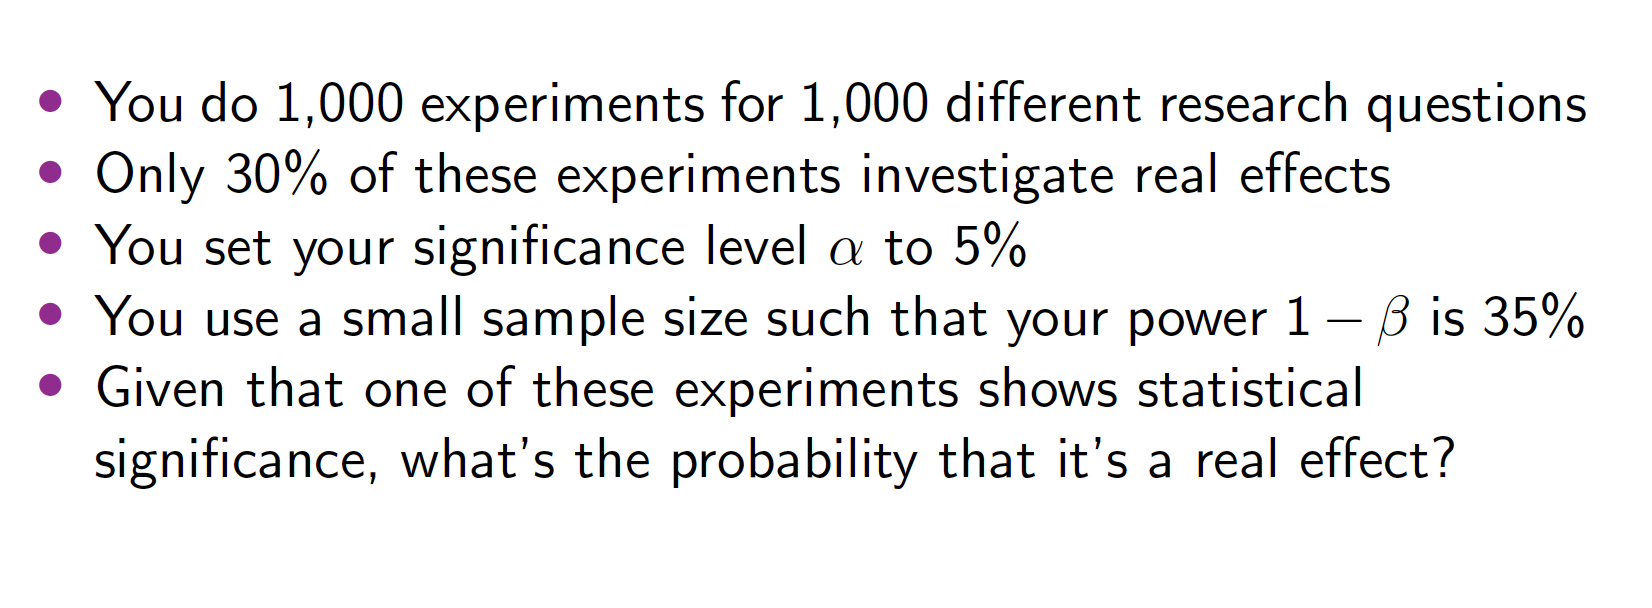
\includegraphics[width=0.5\textwidth]{figures/bayes_problem.png}
    \caption{
       problem from class}
    \label{fig:bayes_problem}
  \end{center}
\end{figure}

The solution is provided below:

\begin{figure}[ht]
  \begin{center}
    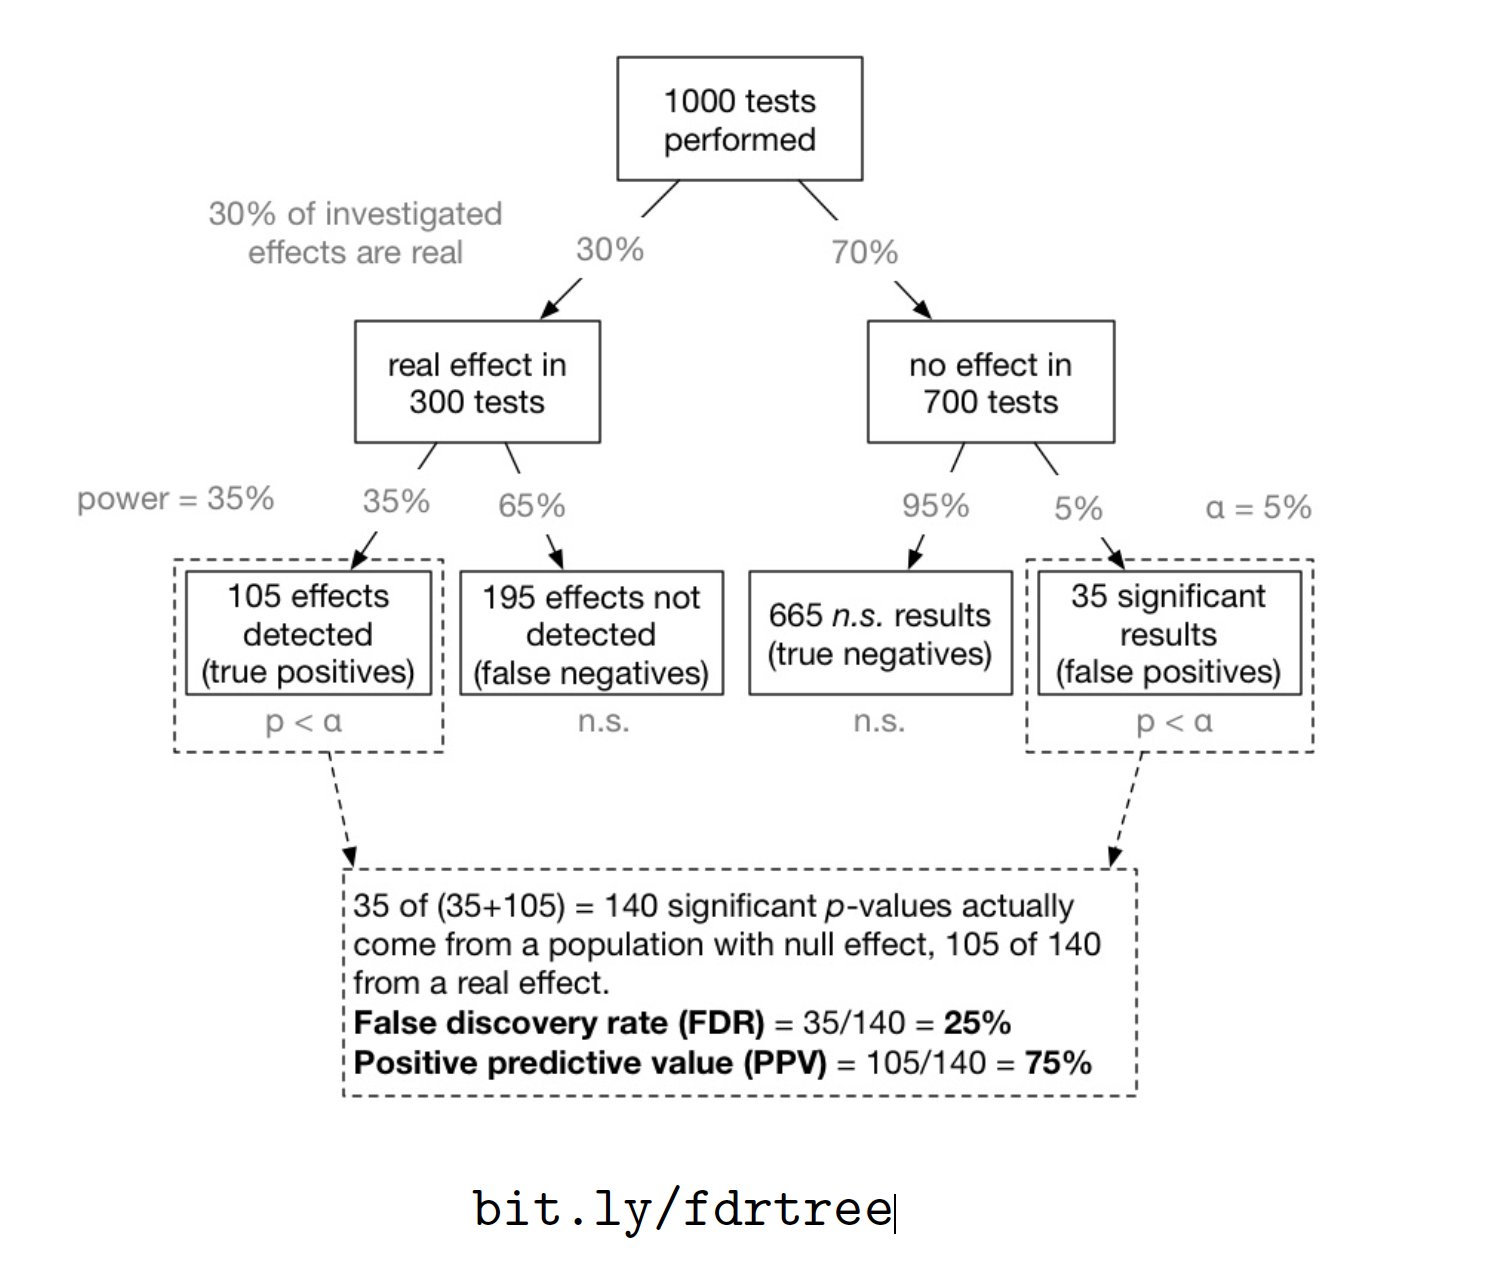
\includegraphics[width=0.5\textwidth]{figures/bayes_solution.png}
    \caption{
       solution from class}
    \label{fig:bayes_solution}
  \end{center}
\end{figure}

When doing this power it's important to remember the following when utilizing Bayes' Rule:

$$ 1 - \beta = \textrm{Power} = \textrm{P(stat sig | real effect)}$$
$$ \alpha = \textrm{P(stat sig | not real effect)}$$
$$ \textrm{False Discovery Rate} = \textrm{P(not real effect | stat sig)}$$

\section{Area Under the Curve and Effect Sizes}

We then analyzed the Area Under the Curve (AUC) which is also referred as the probability of superiority, which counts the fraction of times that the treatment is greater than the control over samples. 

\section{P-Hacking}

We took a look at two studies on Musical Contrast and subjective age as well as musical contrast and chronological rejuvenation. We discussed the studies weaknesses which included poorly defined variables, lack of well defined controls, and strange adjustments to the data to justify normality. We highlighted the studies' P-Hacking issues. P-Hacking is well explained with an interactive graphic in \url{https://fivethirtyeight.com/features/science-isnt-broken/#part1} and suggests some methods for better scientific research practices in the future. Broadly speaking, p-hacking is the process of looking at as many sources of data as possible and searching for any statistically significant result and publishing the results accordingly. Within the FiveThirtyEight applet, we can see that changing the factors can lead to broad generalizations such as Democrats or Republicans having large effects on the economy, when in reality, the situation is more complicated and can't be understood by just one data set with perfectly selected data to meet publishing criteria. 

\begin{figure}[ht]
  \begin{center}
    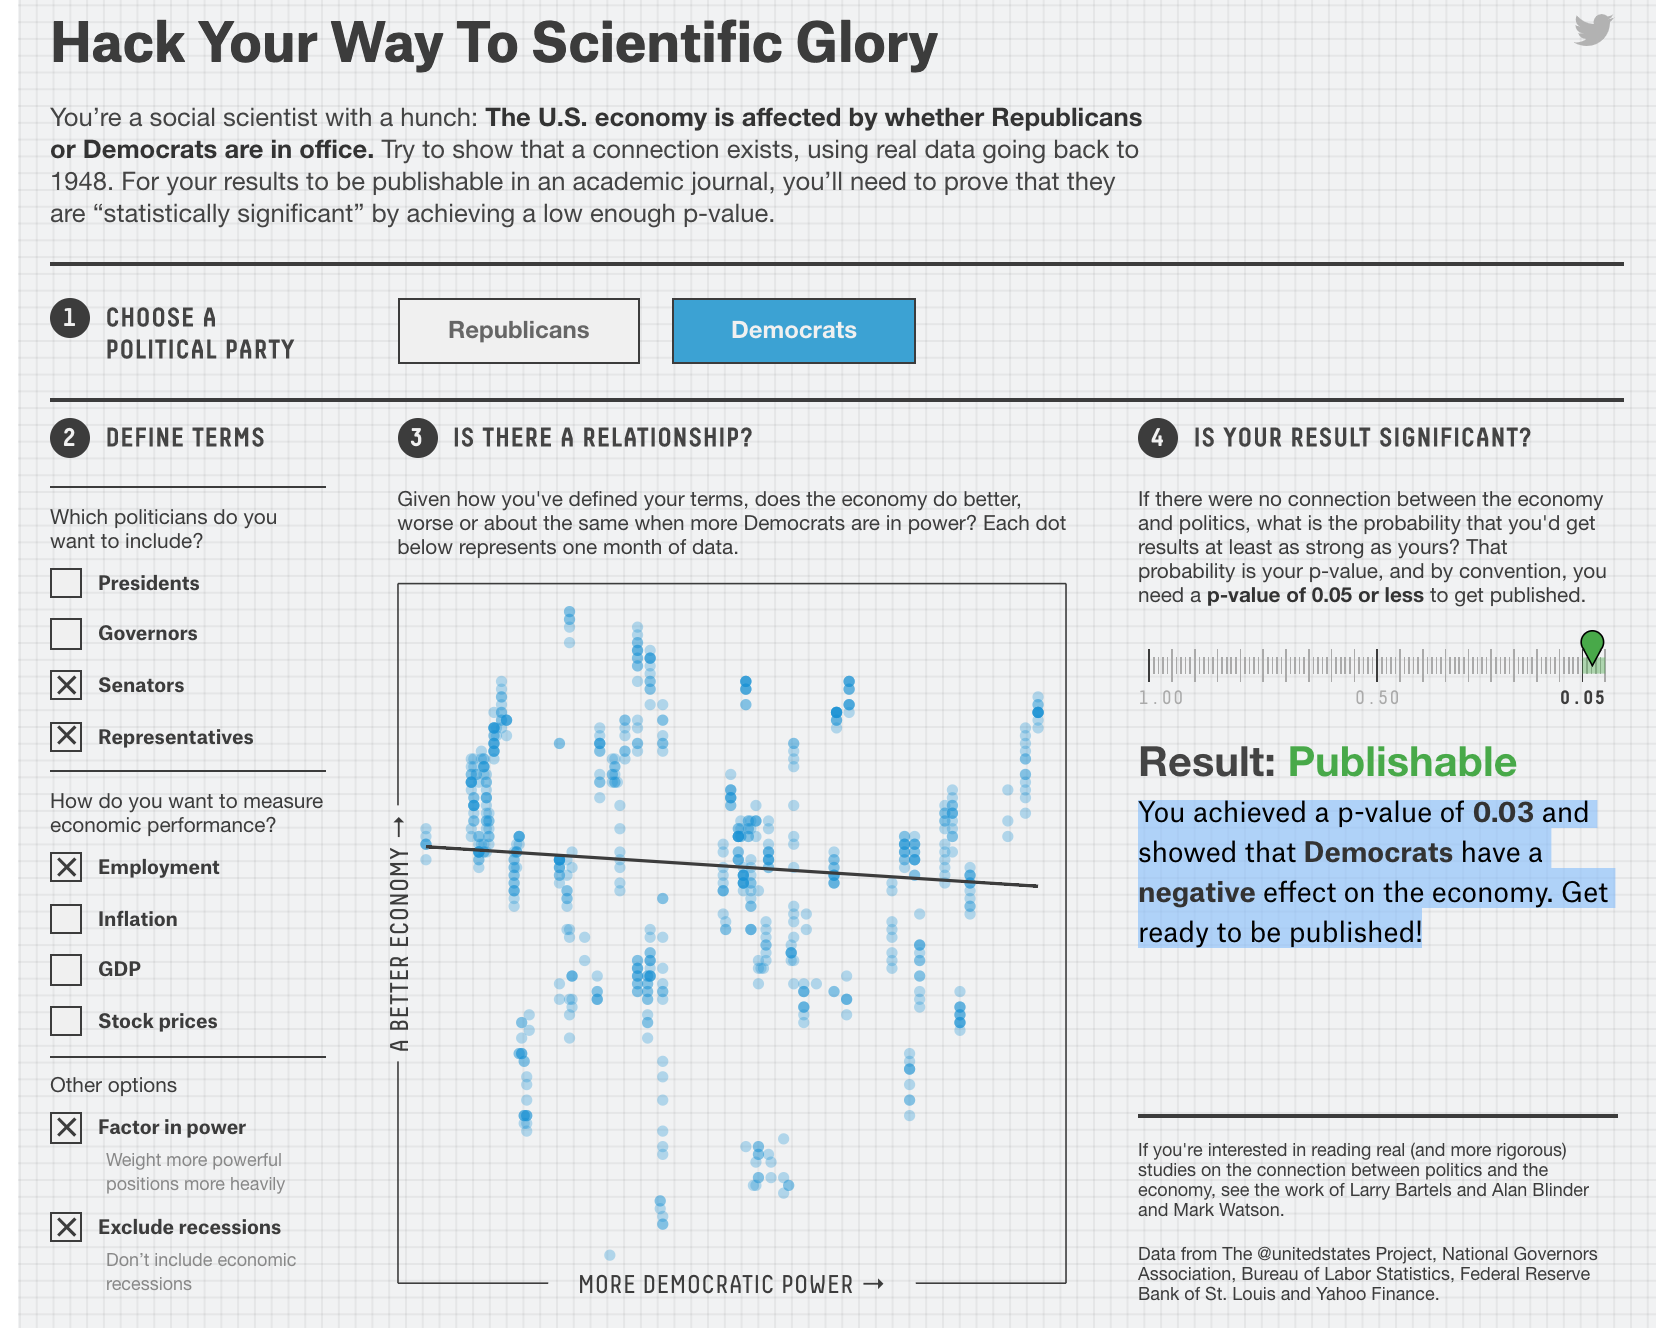
\includegraphics[width=0.5\textwidth]{figures/p_hack.png}
    \caption{
	FiveThirtyEight p-hack} 
    \label{fig:p_hack}
  \end{center}
\end{figure}

We considered the XKCD comic \url{xkcd.com/882}. In this hypothetical, researchers looked at acne trends and jelly bean consumption. 

\section{Publication and Citation Bias}

Lastly, we looked at the effects of a culture where scientists are icentivized to only pubish positive results. Specifically, even though 50\% of FDA registered studies find positive results, 95\% of publications report positive findings. More information is here: \url{bit.ly/depressionspin}.

\section{Conclusion}

Think about the following questions:

\begin{itemize}
    \item Was the research done and reported honestly and correctly?
    \item Is the result real or an artifact of the data or analysis of the data?
    \item Will the results hold up over time?
    \item How robust is the result to small changes?
    \item How important or useful is the finding? 
\end{itemize}
